\subsection{Arbres de décisions}

\paragraph{}
Nous avons décidé d'utiliser comme second algorithme celui des arbres de décisions. Cet algorithme, bien que très complexe à mettre en place, nous permet d'obtenir des résultats faciles à interpréter et en très visuelles.
Vu la difficulté d'implémentation de cet algorithme nous en avons donc chercher un déjà réaliser pour le comprendre et l'utiliser avec nos fichiers de tests. C'est pourquoi nous utilisons l'algorithme jaDTi un algorithme en Java qui implémente les arbres de décisions, et, qui est libre et disponible sur Internet (General Public License) sur http://www.run.montefiore.ulg.ac.be/~francois/software/jaDTi/.


\subsubsection{Le principe}

\paragraph{}
Les arbres de décisions, qui font parties des méthodes d'apprentissage supervisé,  permettent  de réunir en un seul arbres toutes les classes traités. Chaque classes est représenté par une feuille de l'arbre. Les nœuds présent dans l'arbre représentent, quant à eux, les différents sélecteurs pour choisir au mieux dans quel fils il faut se diriger pour classer l'objet traité. C'est pourquoi le choix du sélecteur ou variable de segmentation est vraiment important pour l'efficacité des résultats obtenus.  
Plusieurs algorithmes permettent de construire des arbres de décisions. Ils  décrivent le ou les critères de segmentation, les méthodes d'élagages et aussi  les manières de gérer les données manquantes.
Dans l'algorithme que nous utilisons c'est l'algorithme C4.5 qui est implémentés pour la construction de l'arbre. C'est un algorithme de classification supervisé, publié par Ross Quinlan. Il se base sur une mesure de l'entropie dans l'échantillon d'apprentissage pour choisir le sélecteur de chaque nœud.

\paragraph{}
Dans notre sujet,  les classes (feuilles) obtenus représentent nos différents "Topics",  et ainsi  les décisions de classifications en fonctions des mots trouvés restent visibles en parcourant la branche concernée.
Ici l'algorithme d'apprentissage nous permet d'obtenir un arbre qui contient donc nos "Topics" au niveau des feuilles et chaque nœud contient un mot qui permet de choisir vers quel fils on se déplace en fonction de si l'article contient ou non le mot.  


\subsubsection{Utilisation de l'algorithme}

\paragraph{Mise en forme des données}  
Dans un premier temps, pour pouvoir utiliser cet algorithme, nous avons du mettre nos données sous la forme suivante :

object name "TOPICS" symbolic "TOPICS" symbolic ...
"id de l'article" yes no ... "mots1"
"id de l'article" no yes ... "mots2"
"id de l'article" no no ... "mots3"

Tous les mots (raciniser et avec les mots inutiles supprimés) sont ajoutés (yes/no) aux différentes classes (tous les différents"TOPICS") en fonction de si ils apparaissent ou non dans ce topic.
La première ligne de ce fichier contient donc tous les topics présents avec leurs types (ici ils sont tous symbolic). Et les lignes suivantes contiennent pour chaque mots de chaque article s'il apparait ou non dans les topics correspondants.
Nous obtenons ce fichier à l'aide d'un script Perl que nous avons écris. Ce fichier, au vu du nombre important d'articles dans notre jeu de données est très volumineux. Nous obtenons donc notre fichier de données d'entrainement pour pouvoir utiliser l'algorithme d'arbre de décision.

\paragraph{Modification de l'algorithme}  
Nous n'avons pas eu besoin de faire d'importantes modifications pour utiliser cette algorithme. En effet, nous avons seulment modifié et ajouté quelques lignes de code pour améliorer l'affichage de sortie et permettre de visualiser plus facilement les résultats.

\paragraph{Affichage des résultats}
Dans l'algorithme une classe est disponible "DecisionTreeToDot" pour permettre de générer un fichier .dot qui représente l'arbre obtenus. Nous pouvons ensuite visualiser cet arbre grâce à "graphviz"
L'arbre généré ici est très grand et ne permet pas de l'ajouter en intégralité dans ce rapport c'est pourquoi nous ne présenterons qu'un petit bout de cet arbre pour pouvoir en extraire facilement le principe. 

Voici donc une partie de l'arbre que nous obtenons :

\begin{figure}[h]									%
\centering										%
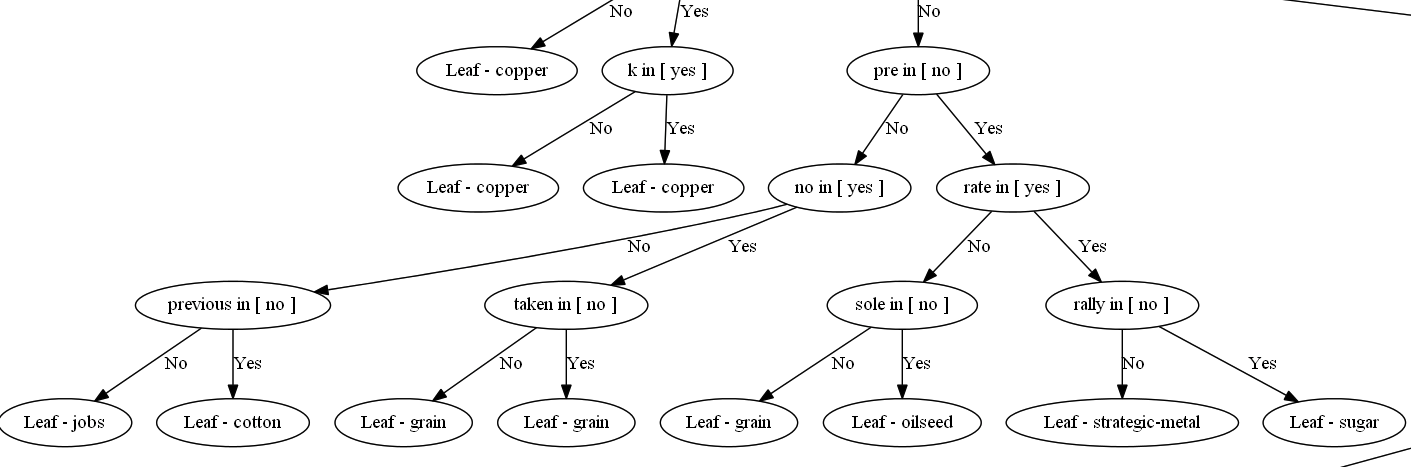
\includegraphics[width=95mm]{./arbre.png}	%
\caption{Une partie de l'arbre obtenue}		%
\label{deviceWindow}								%
\end{figure}

